\section{Method}
%Paragraph one: Overview of the method. What are the high level steps taken to build the system? What are the key techniques used within the system?
We identify split errors in the segmentation using a convolutional neural network (CNN). The network is designed to scan existing boundaries in the segmentation and provide a score on how likely this edge causes a split error. We use this trained CNN in the detection and correction of split errors as well as merge errors as follows.

For split errors we classify existing boundaries in the segmentation according to if they cause a split error or not. Detecting a split error boundary automatically allows to correct the split error by removing the detected edge and thus by merging the two split regions into one correct segment. 

Identification and correction of merge errors is challenging, because the correction of a merge error requires the generation of a new edge in the segmentation, which was missed by the automatic segmentation before. To address this problem we generate 20 potential boundary candidates and classify these using the inverse score of the designed network for split error detection. This means, if the CNN detects a boundary with a very low split error score, such boundary is a candidate for a merge error.

\begin{figure}[t]
\centering
\includegraphics[scale=.15]{gfx/patches.pdf}
\caption{Show visually each of the inputs to the system on a couple of patches.}
\end{figure}


\subsection{Network Design}
%Paragraph: What is the rationale behind our network design? Why do we think this will work over other approaches? 
We train a CNN to detect split errors in the segmentation. In contrast to the standard CNNs, which are the state of the art for membrane detection and automatic segmentation of electron microscopy images of brain tissue, the network trained to detect split errors takes a wider context window and multiple input channels into account. The input channels correspond to different outputs of the automatic segmentation like the boundary probability map and binary masks corresponding to segmented regions and region overlaps. The network can then leverage these multiple input patches to identify and correct errors made by the previous membrane detection network and the automatic segmentation pipeline. 

%Paragraph: What are the inputs to the design? What is the design? Parameters of the design.
The design of the network follows the design of Viren et al. \VKF{Cite Viren}, who designed a network for agglomerative clustering of oversegmentations. In contrast to Jain et al, our network operates on 2D patches instead of 3D volumes. Operating in 2D gives the advantage that we do not require images to be aligned as an image stack which is computational expensive. 

The input to the network consists of several input patches. The original design of Jain et al. included a patch from the electron microscopy image, a membrane probability map generated for the initial automatic segmentation, and a binary mask of the two regions of the potential split error. Our modified design also includes the label boundary in two variations.
Each of the input patches is connected to a 2-layer network, with each layer consisting of a convolutional and a pooling layer as shown in figure \ref{fig:layers}. The output of all these networks is then combined by a fully connected MLP with one hidden layer and a two class logistic regression output layer. 

Jain et al. also developed two pooling techniques employed in the pooling layers of the CNN, dynamic boundary pooling and dynamic object pooling. The idea is to focus the pooling output on regions of interest, like the boundary between two regions (boundary pooling), or the joint area of the two regions considered (object pooling). Instead of conventional pooling where a sliding window is equally applied to the whole output of the convolutional layer, dynamic pooling only averages outputs within the region of interest. We implemented both pooling methods and compare them in table \VKF{reference to result table}.

\begin{figure}[t]
 \centering
    \subfloat[CNN Layers\label{fig:layers}]{%
      \includegraphics[width=0.55\textwidth]{gfx/layers.pdf}
    }
    \hfill
    \subfloat[Network configurations\label{fig:networks}]{%
      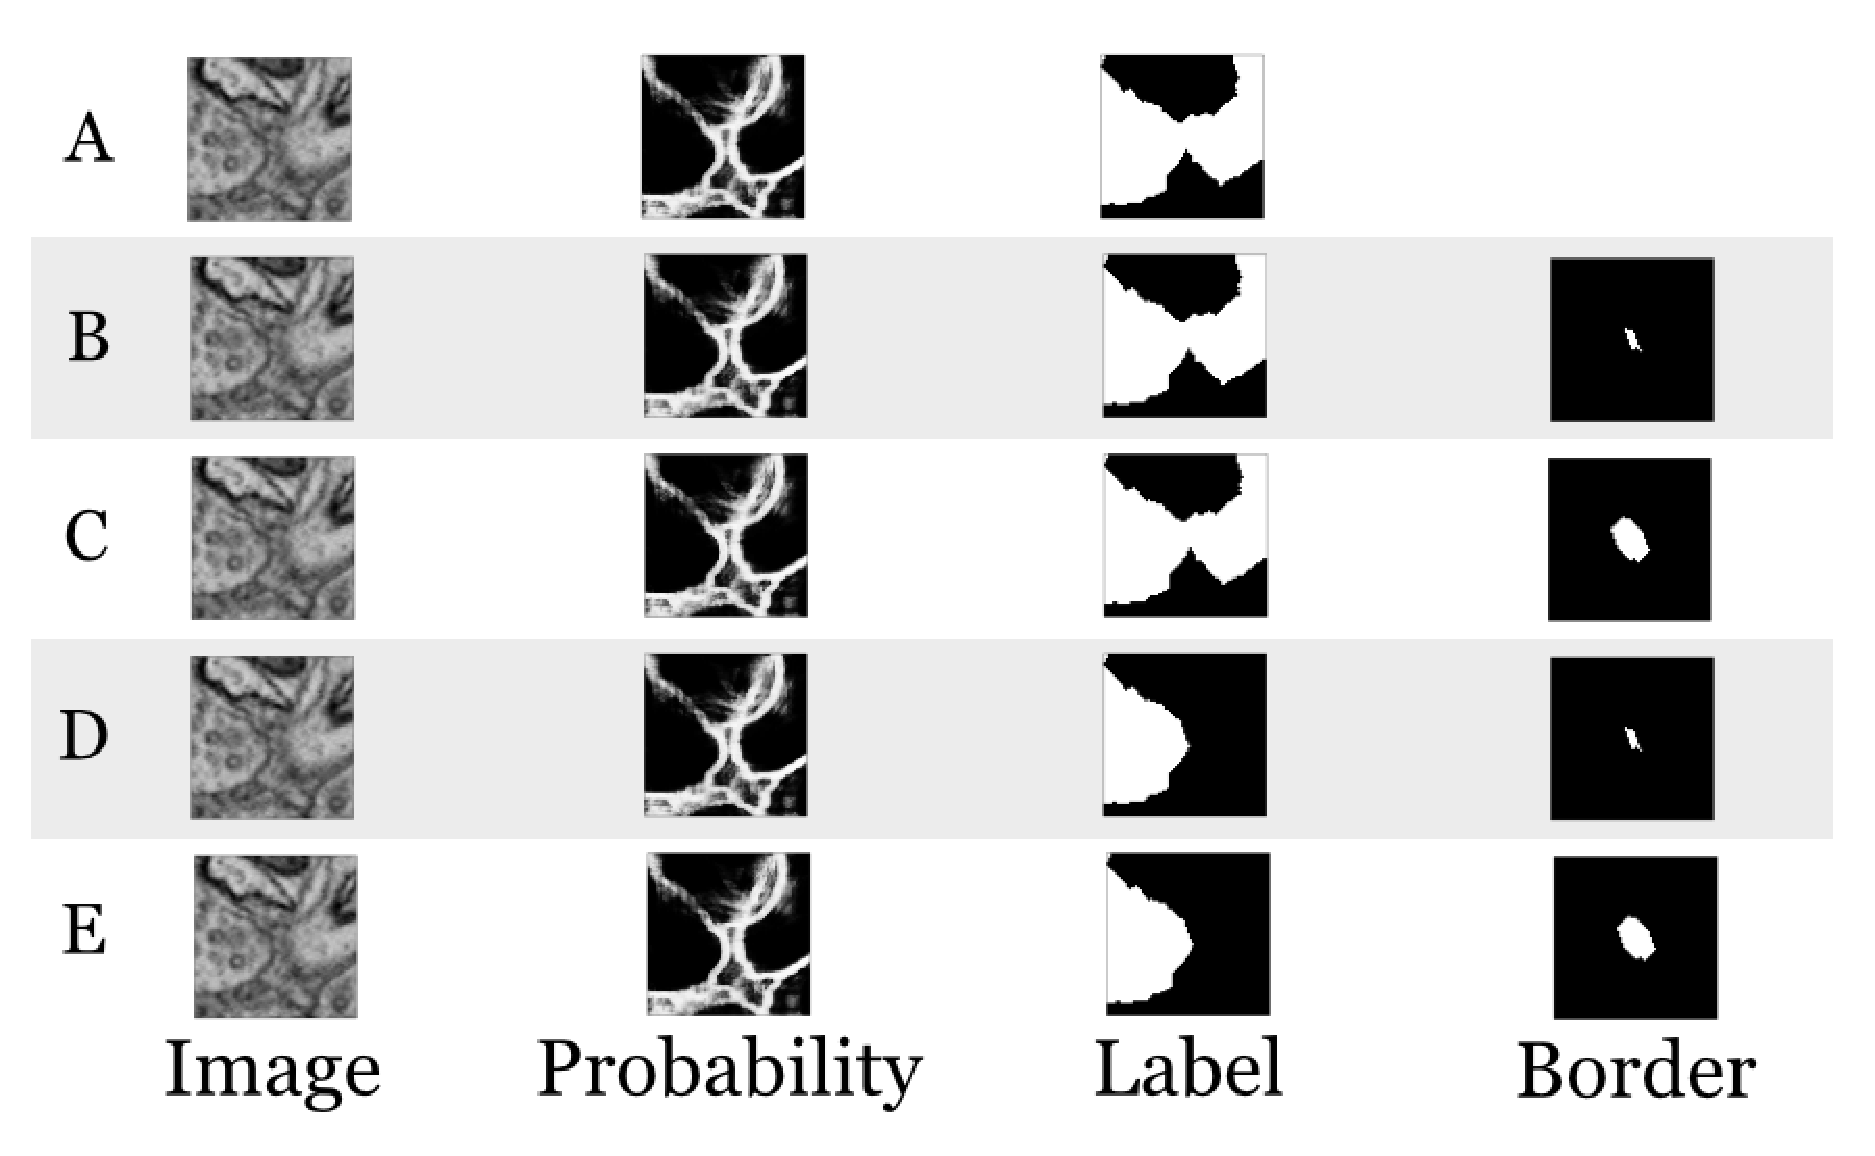
\includegraphics[width=0.4\textwidth]{gfx/networks.pdf}
    }
	\caption{a) Our proposed network architecture with up to four input channels. Each input channel involves two convolutional and two pooling layers with optional dynamic pooling using a binary mask as described by Bogovic et al \cite{viren}. b) We trained five different network configurations with three and four inputs: A) image, probability and merged binary mask, B) extended with a small border mask, C) extended with a large border mask and D)+E) using a single label binary mask instead of the merged one with the small and large border mask.}
\end{figure}
%  
%    \begin{subfig}[b]{0.5\textwidth}
%        \includegraphics[scale=.15]
%        \caption{CNN Layers}
%        \label{fig:layers}
%    \end{subfigure}
%    \begin{subfigure}[b]{0.5\textwidth}
%        \includegraphics[scale=.15]
%        \caption{Different Network Configurations}
%        \label{fig:networks}
%    \end{subfigure}    
%\missingfigure{Network architecture figure}



\subsection{Training}

To train the network, we used a dataset of a mouse cortex (1024x1024x75 pixels). The tissue is dense mammalian neuropil from layers 4 and 5 of the S1 primary somatosensory cortex of a healthy mouse. The resolution of our data set is 6nm/pixel and the section thickness is 30nm. We trained an automatic segmentation pipeline on a similar dataset and used it to segment the data \cite{rhoana}. Manually labeled expert segmentation was available as a ground truth for the entire dataset. We used the first 65 sections of the data for training, the next 5 for validation and the last 5 for testing.

We generated 

We used a publicly available dataset of a mouse cortex (1024x1024x65 pixels) for 

Paragraph: How did we train the network? What tricks did we employ (e.g., rotation)? What are the parameters of the training? What software stack did we use? Hardware platform, training time (none very interesting, but for completeness). When do we stop training?



Paragraph: What are the thresholds in the system? How do we pick the thresholds?


\begin{table}
\begin{tabular}{ll}
\toprule
Parameter & Value \\
\midrule
one & \\
two & \\
three & \\
\bottomrule
\end{tabular}
\caption{This is a table of parameters. This is not very interesting, but it's easier to read than in the body text and putting everything together helps the reader quickly assess.}
\end{table}